
%%%%%%%%%%%%%%%%%%%%%%%%%%%%%%%%%%%%%%%%%%%% Articolo - A4 - Portrait


%%%%%%%%%%%%%%%%%%%%%%%%%%%%%%%%%%%%%%%%%%%% preambolo

\documentclass[10pt]{article}

%%%%%%%%%%%%%%%%%%%%%%%%%%%%%%%%%%%%%%%%%%%% packages
%\usepackage[T1]{fontenc}
\usepackage[latin1]{inputenc}
\usepackage[italian]{babel}
\usepackage{multicol}
\usepackage{amsthm}
\usepackage{caption}
\captionsetup{justification=raggedright, singlelinecheck = false}
\setlength{\columnsep}{1cm}

\usepackage[margin=1in]{geometry}
\usepackage{amsfonts, amsmath, amssymb}
\usepackage[none]{hyphenat}
\usepackage{fancyhdr}
\usepackage{graphics}
\usepackage{lipsum}
\usepackage{float}
\usepackage[nottoc, notlot, notlof]{tocbibind}
\usepackage{pgf, tikz, pgfplots} 
\pgfplotsset{compat=1.15}
\usepackage{mathrsfs}
\usetikzlibrary{arrows, calc}

\newtheorem{theorem}{Teorema}[section]
\newtheorem{corollary}{Corollario}[theorem]
\newtheorem{lemma}[theorem]{Lemma}
\theoremstyle{definition}
\newtheorem{definition}{Definizione}[section]
\theoremstyle{remark}
\newtheorem*{remark}{Osservazioni}

%%%%%%%%%%%%%%%%%%%%%%%%%%%%%%%%%%%%%%%%%%%% stile pagina

\pagestyle{fancy}
\fancyhead{}
\fancyfoot{}
\fancyhead[L]{\small \MakeUppercase{lezioni di matematica per il Liceo}}
\fancyhead[R]{\small \emph{prof. Diego Fantinelli}}
\fancyfoot[C]{\thepage}
\renewcommand{\headrulewidth}{0.5pt}
\renewcommand{\footrulewidth}{0.1pt}

\parindent 0ex
\setlength{\parindent}{0em}
\setlength{\parskip}{0em}
\renewcommand{\baselinestretch}{1.5}
\newcommand{\E}{\mathrm{e}}

%%%%%%%%%%%%%%%%%%%%%%%%%%%%%%%%%%%%%%%%%%%% title page

\begin{document}

\begin{titlepage}
\begin{center}
\vspace*{1cm}

\Large{\textbf{Dipartimento di Matematica}}\\
\large{\textbf{- diego fantinelli -}}\\
\vfill
\line(1,0){400}\\[.5mm]
\huge{\textbf{Lezioni di Matematica per il Liceo}}\\[3mm]
\Large{\textbf{- Sottotitolo:  -}}\\[1mm]
\line(1,0){400}\\
\vfill
%{\scriptsize By Student Name}\\
%{\scriptsize Candidate \#} \\
%{\scriptsize \today} \\

\end{center}
\end{titlepage}

%%%%%%%%%%%%%%%%%%%%%%%%%%%%%%%%%%%%%%%%%%%% introduzione

\tableofcontents
\thispagestyle{empty}
\clearpage

\setcounter{page}{1}

\section{Introduzione}
Il presente documento contiene le principali soluzioni per la formattazione di un testo scientifico, con particolare riferimento ai testi matematici, comprensivi di \emph{formule}, e caratteri speciali

\subsection{Come recuperare l'autostima}
Sed fringilla, neque sit amet maximus luctus, neque eros fermentum ipsum, nec hendrerit leo urna id urna. Pellentesque vel odio lobortis diam placerat porttitor non auctor leo.\\

\begin{multicols}{2}

\subsection{Formule in testo \emph{multicolonne}}
Orci varius natoque penatibus et magnis dis parturient montes, nascetur ridiculus mus. Integer pretium bibendum dolor eget interdum.\\[3mm]
\noindent
\vspace{10pt}
\begin{tikzpicture}
\begin{axis}[
    xmin=-11,xmax=11,
    ymin=-11,ymax=11,
    grid=both,
    grid style={line width=.1pt, draw=gray!10},
    major grid style={line width=.2pt,draw=gray!50},
    axis lines=middle,
    minor tick num=5,
    enlargelimits={abs=0.5},
    axis line style={-latex},
    ticklabel style={font=\tiny,fill=white},
    xlabel style={at={(ticklabel* cs:1)},anchor=north west},
    ylabel style={at={(ticklabel* cs:1)},anchor=south west}
]

\coordinate (O) at (0,0);
\node[fill=white,circle,inner sep=0pt] (O-label) at ($(O)+(-135:10pt)$) {};

\end{axis}
\end{tikzpicture}
\\
Sed ultrices mi a lacus vestibulum aliquet. Nam tincidunt dui in pellentesque hendrerit. Phasellus diam libero, laoreet eu varius sed, vulputate a orci. Etiam odio tortor, sagittis nec quam quis, iaculis ultrices purus. Nunc semper purus nec elit mattis.\\[4mm]
$\displaystyle{\lim \limits_{x \to \infty} \frac{f(b)-f(a)}{x-a}=f'(a)}$\\[4mm]
Sed ultrices mi a lacus vestibulum aliquet. Nam tincidunt dui in pellentesque hendrerit. Phasellus diam libero, laoreet eu varius sed, vulputate a orci. Etiam odio tortor, sagittis nec quam quis, iaculis ultrices purus. Nunc semper purus nec elit mattis.\\
\begin{equation}
	\displaystyle{\int_a^b{f(x) \,dx=\lim \limits_{x \to \infty} \sum \limits_{k=1}^{n}f(x_k) \cdot \Delta x}}
\end{equation}\\
Sed ultrices mi a lacus vestibulum aliquet. Nam tincidunt dui in pellentesque hendrerit. Phasellus diam libero, laoreet eu varius sed, vulputate a orci. Etiam odio tortor, sagittis nec quam quis, iaculis ultrices purus. Nunc semper purus nec elit mattis.
\begin{align*}
x&=y           &  w &=z              &  a&=b+c\\
2x&=-y         &  3w&=\frac{1}{2}z   &  a&=b\\
-4 + 5x&=2+y   &  w+2&=-1+w          &  ab&=cb
\end{align*}
\\[1.5mm]
\end{multicols}

%%%%%%%%%%%%%%%%%%%%%%%%%%%%%%%%%%%%%%%%%%%% sez. 2
\newpage
\section*{Classi Prime}
\hrule 
\vspace{24pt}
\lipsum[1]
\vspace{24pt}
\section{Classi Prime}

\lipsum[2]
\subsection{Gli Insiemi Numerici}
Lorem ipsum dolor sit amet, consectetur adipiscing elit. Sed varius lacus eget magna elementum, quis ultricies justo vestibulum. Proin sed dolor vel est rhoncus tristique iaculis auctor mauris.\\[3mm]
$f(x)=(x-3)^2+ \displaystyle \frac{x}{2}$ ha dominio $\mathrm{D}_f:(-\infty,+\infty)$
e range $\mathrm{R}_f:\left[\frac{1}{2},\infty\right)$.

\subsubsection{I Numeri Naturali}

\subsubsection{L'Insieme Z dei Numeri Razionali}

\begin{align*}
x&=y           &  w &=z              &  a&=b+c\\
2x&=-y         &  3w&=\frac{1}{2}z   &  a&=b\\
-4 + 5x&=2+y   &  w+2&=-1+w          &  ab&=cb
\end{align*}

\subsection{Come inserire le formule matematiche}
Lorem ipsum dolor sit amet, consectetur adipiscing elit. Sed varius lacus eget magna elementum, quis ultricies justo vestibulum. Proin sed dolor vel est rhoncus tristique iaculis auctor mauris.\\[3mm]
$f(x)=(x-3)^2+ \displaystyle \frac{x}{2}$ ha dominio $\mathrm{D}_f:(-\infty,+\infty)$
e range $\mathrm{R}_f:\left[\frac{1}{2},\infty\right)$.\\


%%%%%%%%%%%%%%%%%%%%%%%%%%%%%%%%%%%%%%%%%%%% sez. 3


\newpage
\section{ Second Anno}

\begin{multicols}{2}
\lipsum[1]

\end{multicols}
\subsection{Come inserire le formule matematiche}
Lorem ipsum dolor sit amet, consectetur adipiscing elit. Sed varius lacus eget magna elementum, quis ultricies justo vestibulum. Proin sed dolor vel est rhoncus tristique iaculis auctor mauris.\\[3mm]
$f(x)=(x-3)^2+ \displaystyle \frac{x}{2}$ ha dominio $\mathrm{D}_f:(-\infty,+\infty)$
e range $\mathrm{R}_f:\left[\frac{1}{2},\infty\right)$.\\

%$\displaystyle{\lim \limits_{x \to \infty} \frac{f(b)-f(a)}{x-a}=f'(a)}$\\[1cm]

\subsubsection{Il Calcolo Letterale: L'Algebra}

%%%%%%%%%%%%%%%%%%%%%%%%%%%%%%%%%%%%%%%%%%%% Equazioni utilizzando equation

\begin{equation}
	\displaystyle{\lim \limits_{x \to \infty} \frac{f(b)-f(a)}{x-a}=f'(a)}
\end{equation}\\[1cm]
\emph{integrali}
\begin{equation}
	\displaystyle{\int \limits_{a}^{b}x^2 \,dx=\left[\frac{x^3}{3}\right]_{a}^{b}=\frac{b^3}{3}-\frac{a^3}{3}}
\end{equation}\\[1cm]
\emph{Sommatorie}
\begin{equation}
	\displaystyle{\sum \limits_{n=1}^{\infty}ar^n=a+ar+ar^2+\cdots+ar^n}
\end{equation}\\[1cm]
\emph{Mix}
\begin{equation}
	\displaystyle{\int_a^b{f(x) \,dx=\lim \limits_{x \to \infty} \sum \limits_{k=1}^{n}f(x_k) \cdot \Delta x}}
\end{equation}\\[1cm]
\emph{Vettori}
\begin{equation}
	\displaystyle{\vec{v}=v_1 \vec{i}+v_2 \vec{j}=\langle v_1, v_2 \rangle}
\end{equation}

%%%%%%%%%%%%%%%%%%%%%%%%%%%%%%%%%%%%%%%%%%%% tabelle e arrays

\section{Tabelle}
%\begin{figure}[h!]
%Nam tincidunt dui in pellentesque hendrerit. Phasellus diam libero, laoreet eu varius sed, vulputate a orci. Etiam odio tortor\\[5mm]
%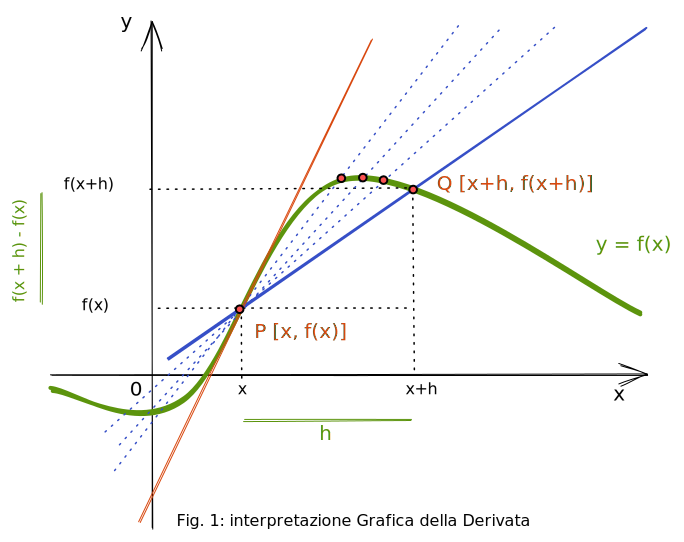
\includegraphics[width=0.7\textwidth]{Derivata}
%\caption {\textit{Esempio di Rappresentazione grafica della derivata di una funzione}}
%\end{figure}
\noindent
Nam tincidunt dui in pellentesque hendrerit. Phasellus diam libero, laoreet eu varius sed, vulputate a orci. Etiam odio tortor, sagittis nec quam quis, iaculis ultrices purus. Nunc semper purus nec elit mattis.\\

	\subsection{Tabelle e Arrays}
	\begin{table}[H]
%	\centering
	\caption{Relazione tra $f$ e $f'$.}
	\def\arraystretch{1.5}
	\begin{tabular}{c|c|r} % con |c| si definiscono le colonne e poi si separano le righe tra loro con \hline

	{$f(x)$} & {$f'(x)$}\\ \hline
	$x>0$ & La funzione $f(x)$ � \emph{crescente}. & prova 1\\
	\hline
	$x<0$ & La funzione $f(x)$ � \emph{decrescente}. & prova 2\\
	\hline	
	$x<0$ & La funzione $f(x)$ � \emph{costante}. & prova 3\\	
	\end{tabular}
		
	\end{table}

\section{Alcune \emph {Griglie per grafici}}
\subsection{Come inserire le formule matematiche}
Lorem ipsum dolor sit amet, consectetur adipiscing elit. Sed varius lacus eget magna elementum, quis ultricies justo vestibulum. Proin sed dolor vel est rhoncus tristique iaculis auctor mauris.\\[3mm]
$f(x)=(x-3)^2+ \displaystyle \frac{x}{2}$ ha dominio $\mathrm{D}_f:(-\infty,+\infty)$
e range $\mathrm{R}_f:\left[\frac{1}{2},\infty\right)$.\\

\begin{tikzpicture}
\begin{axis}[
    xmin=-11,xmax=11,
    ymin=-11,ymax=11,
    grid=both,
    grid style={line width=.1pt, draw=gray!10},
    major grid style={line width=.2pt,draw=gray!50},
    axis lines=middle,
    minor tick num=5,
    enlargelimits={abs=0.5},
    axis line style={latex-latex},
    ticklabel style={font=\tiny,fill=white},
    xlabel style={at={(ticklabel* cs:1)},anchor=north west},
    ylabel style={at={(ticklabel* cs:1)},anchor=south west}
]

\coordinate (O) at (0,0);
\node[fill=white,circle,inner sep=0pt] (O-label) at ($(O)+(-135:10pt)$) {};
\end{axis}

\begin{axis}[xshift=9cm,
    xmin=-11,xmax=11,
    ymin=-11,ymax=11,
    grid=both,
    axis lines=middle,
    minor tick num=5,
    enlargelimits={abs=0.5},
    axis line style={latex-latex},
    ticklabel style={font=\tiny,fill=white},
    xlabel style={at={(ticklabel* cs:1)},anchor=north west},
    ylabel style={at={(ticklabel* cs:1)},anchor=south west}
]

\coordinate (O) at (0,0);
\node[fill=white,circle,inner sep=0pt] (O-label) at ($(O)+(-135:10pt)$) {};

\end{axis}
\end{tikzpicture}

\vspace{1cm}

\begin{figure}[h!]
\begin{tikzpicture}
\begin{axis}[
	%xmin=0,xmax=5,
    %ymin=0,ymax=0.6,
    width=\textwidth,
	height=0.5\textwidth,
    grid=both,
    grid style={line width=.1pt, draw=gray!30},
    major grid style={line width=.2pt, draw=gray!50},
    axis lines=middle,
    minor tick num=5,
    enlargelimits={abs=0.5},
    axis line style={-latex},
    ticklabel style={font=\tiny,fill=white},
    xlabel=$x$,
    ylabel=$f(x)$
]

\end{axis}
\end{tikzpicture}
\caption{Griglia per Grafico Generico}
\end{figure}

%%%%%%%%%%%%%%%%%%%%%%%%%%%%%%%%%%%%%%%%%%%% Grafico di una Funzione

\newpage
\section{Grafico grande}

Il mio primo grafico con \emph{referencing} mostrato in Figura:\ref{primo-grafico}

\begin{figure}[h!]
\begin{tikzpicture}
\begin{axis}[
	%xmin=0,xmax=5,
    %ymin=0,ymax=0.6,
    width=\textwidth,
	height=0.5\textwidth,
    grid=both,
    grid style={line width=.1pt, draw=gray!10},
    major grid style={line width=.2pt, draw=gray!50},
    axis lines=middle,
    minor tick num=5,
    enlargelimits={abs=0.5},
    axis line style={-latex},
    ticklabel style={font=\tiny,fill=white},
    xlabel=$x$,
    ylabel=$f(x)$,
	legend entries={
        \small $y = 0.5x\E^{-x}$,
        \small $y=x\E^{-x}$,
        \small $y=2x\E^{-x}$,
        \small $y=3x\E^{-x}$
}
]
	\addplot[
	domain=0:5,
	thick,
	pink
	]
	{0.5*x*exp(-x)};
	
	\addplot[
	domain=0:5,
	thick,
	green
	]
	{x*exp(-x)};
	
	\addplot[
	domain=0:5,
	thick,
	dashdotted,
	blue
	]
	{2*x*exp(-x)};
	
	\addplot[
	domain=0:5,
	thick,
	black,
	dotted
	]
	{3*x*exp(-x)};
	
\end{axis}
\end{tikzpicture}
\caption{Il mio primo grafico}
\label{fig:primo-grafico}
\end{figure}

%---------------------------------------- 5� anno
\newpage
\fancyhead[R]{\small \emph{V ANNO}}
\section{Il Calcolo Integrale}

\subsection{Cenni storici}
\begin{multicols}{2}
\begin{itemize}
	\item L'idea di base del concetto di integrale era nota ad Archimede di Siracusa, vissuto tra il 287 e il 212 a.C., ed era contenuta nel metodo da lui usato per il calcolo dell'area del cerchio o dell'area sottesa al segmento di un ramo di parabola, detto metodo di {\em esaustione}, gi� da Eudosso di Cnido.
	\item Nel XVII secolo alcuni matematici trovarono altri metodi per calcolare l'area sottesa al grafico di semplici funzioni, tra di essi figurano, ad esempio, Bonaventura Cavalieri, scopritore del metodo degli indivisibili (anni 1640), Pierre de Fermat (1636) e Nicolaus Mercator (1668). In quegli stessi anni Pietro Mengoli (1659) diede una prima definizione di integrale.
	\item Nel diciassettesimo e diciottesimo secolo Isaac Newton, Gottfried Leibniz, Johann Bernoulli dimostrarono indipendentemente il teorema fondamentale del calcolo integrale, che ricondusse tale problema alla ricerca della primitiva di una funzione.
\end{itemize}
\end{multicols}

\subsection{La definizione di Integrale}
\begin{itemize}
	\item La definizione di integrale per le funzioni continue in un intervallo venne inizialmente formulata da Augustin-Louis Cauchy, che a partire dal lavoro di Mengoli, descrisse l'integrale utilizzando la definizione di limite.
	\item In seguito Bernhard Riemann propose la sua definizione, in modo da comprendere classi pi� estese di funzioni. Nel 1875, Gaston Darboux riformul� la definizione gi� individuata da Cauchy in modo da evitare l'uso di limiti e dimostrando che era del tutto equivalente alla definizione data da Riemann. Per questo motivo spesso si parla di integrale di Riemann-Darboux.
	\item Allo scopo di comprendere una classe molto pi� estesa di funzioni, Henri Lebesgue produsse una definizione di integrale pi� complessa, attraverso l'introduzione della teoria della misura.
	\item In seguito Thomas Stieltjes fu in grado di generalizzare l'integrale di Riemann introducendo il concetto di funzione integratrice e, con un procedimento del tutto analogo, Johann Radon generalizz� l'integrale di Lebesgue.
	\item Una definizione d'integrale alternativa a quella di Lebesgue-Radon venne fornita da Percy J. Daniell, che la ricav� a partire dall'integrale di Riemann-Stieltjes.
\end{itemize}

\theoremstyle{definition}
\begin{definition}
Una funzione $F(x)$ � una {\bf primitiva} della funzione $f(x)$ definita in un intervallo chiuso $[a,b]$ se $F(x)$ � derivabile in tutto $[a,b]$ e la sua derivata � $f(x)$:\\
\begin{center}
	$F'(x) = f(x)$
\end{center} 
\end{definition}

\begin{theorem}[]
%\label{pythagorean}
Se $F(x)$ � una primitiva di $f(x)$, allora le funzioni $F(x) + c$, con $c$ numero reale qualsiasi, sono {\bf tutte e sole} le primitive di $f(x)$
\end{theorem}

\theoremstyle{definition}
\begin{definition}{Integrale Indefinito}
L'{\em Integrale Indefinito} di una funzione $f(x)$ � l'insieme di tutte le primitive $F(x) + c$ di $f(x)$, con $c\in \mathbb{R}$.\\ Si indica con:

\begin{center}
$\displaystyle \int f(x) dx$
\end{center}

\end{definition}

%\begin{theorem}
%Let $f$ be a function whose derivative exists in every point, then $f$ is 
%a continuous function.
%\end{theorem}
%
%\begin{theorem}[Pythagorean theorem]
%\label{pythagorean}
%This is a theorema about right triangles and can be summarised in the next 
%equation 
%\begin{align}
%	x^2 + y^2 = z^2
%\end{align} 
%\end{theorem}
%
%And a consequence of theorem \ref{pythagorean} is the statement in the next 
%corollary.
%
%\begin{corollary}
%There's no right rectangle whose sides measure 3cm, 4cm, and 6cm.
%\end{corollary}
%
%You can reference theorems such as \ref{pythagorean} when a label is assigned.
%
%\begin{lemma}
%Given two line segments whose lengths are $a$ and $b$ respectively there is a 
%real number $r$ such that $b=ra$.
%\end{lemma}
%
%\begin{remark}
%This statement is true, I guess.
%\end{remark}
%
%And the next is a somewhat informal definition
%

\end{document}
